\documentclass[12pt, twoside]{article}
\usepackage[francais]{babel}
\usepackage[T1]{fontenc}
\usepackage[latin1]{inputenc}
\usepackage[left=5mm, right=5mm, top=5mm, bottom=5mm]{geometry}
\usepackage{float}
\usepackage{graphicx}
\usepackage{array}
\usepackage{multirow}
\usepackage{amsmath,amssymb,mathrsfs}
\usepackage{textcomp}
\pagestyle{empty}
\usepackage{soul}

\begin{document} 

NOM PRENOM: \ldots \ldots \ldots \ldots \ldots

\begin{center}
{\fbox{$4^{e}3$ \qquad \qquad \textbf{\Large{Devoir surveill� 6 (sujet 1)}}
\qquad \qquad 15/04/2014}}
\end{center}

\enskip


\textit{\ul{Remarque}: Les exercices 1 et 2 sont � faire sur la photocopie, les
autres sur votre copie.}

\enskip

\ul{\textbf{Exercice 1}}: (\textit{2 points})
\thinspace
Compl�ter le tableau suivant en arrondissant les valeurs au dixi�me.

\begin{center}
\begin{tabular}{|l|c|c|c|c|}
\hline
Angle & 35� & \ldots \ldots & 60� & \ldots \ldots \\
\hline

Cosinus & \ldots \ldots & 0,3 & \ldots \ldots & 0,98 \\
\hline
\end{tabular}
\end{center}

\bigskip

\ul{\textbf{Exercice 2}}: (\textit{2 points})
\thinspace 
Pour chaque question, coche la (ou les ) bonne(s) r�ponse(s).


\begin{center}
\begin{tabular}{|l|c|c|c|}
\hline


Dans un triangle ABC rectangle en A, le c�t� adjacent � l'angle $\widehat{ABC}$
est 

& [AB] & [AC] & [BC] \\

\quad & \fbox{\thinspace} & \fbox{\thinspace} & \fbox{\thinspace} \\

\hline

\quad & \quad & \quad & \quad \\
Dans un triangle DEF rectangle en E, $cos(\widehat{EFD})$ est �gal � 

& $\dfrac{FD}{FE}$ & $\dfrac{ED}{FD}$ & $\dfrac{FE}{FD}$ \\

\quad & \fbox{\thinspace} & \fbox{\thinspace} & \fbox{\thinspace} \\

\hline
\quad & \quad & \quad & \quad \\
Dans ce triangle rectangle, on peut calculer la valeur excate de 

& HF & HG & $\widehat{FHG}$ \\

\quad & \fbox{\thinspace} & \fbox{\thinspace} & \fbox{\thinspace} \\

\hline
\end{tabular}
\end{center}


\bigskip




\ul{\textbf{Exercice 3}}: (\textit{2 points})



\begin{tabular}{cc}
\begin{minipage}{14cm}
Calculer la longueur DF. On donnera une valeur arrondie au millim�tre.
\end{minipage}
&
\begin{minipage}{5cm}
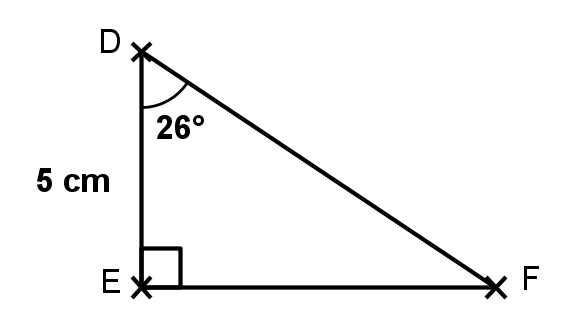
\includegraphics[width=4cm]{images/ex3-sujet1.png}
\end{minipage}
\end{tabular}



\bigskip



\ul{\textbf{Exercice 4}}: (\textit{4 points})


\begin{tabular}{cc}
\begin{minipage}{14cm}
\begin{enumerate}
  \item Calculer la longueur GH. On donnera une valeur arrondie au centim�tre.
  \item Calculer la longueur HI. On donnera une valeur arrondie au centim�tre.
\end{enumerate}
\end{minipage}
&
\begin{minipage}{5cm}
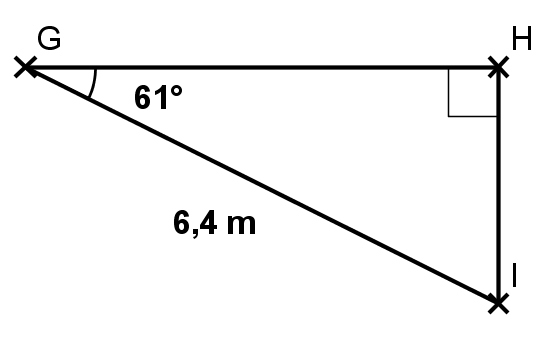
\includegraphics[width=4cm]{images/ex4-sujet1.png}
\end{minipage}
\end{tabular}


\bigskip



\ul{\textbf{Exercice 5}}: (\textit{3 points})

\enskip

KLM est un triangle rectangle en K v�rifiant KL=6km et LM=11km.
\begin{enumerate}
  \item Calculer la mesure de l'angle $\widehat{KLM}$. On donnera une valeur
  arrondie au degr�.
  \item En d�duire une mesure de l' angle $\widehat{KML}$. 
\end{enumerate}


\bigskip



\ul{\textbf{Exercice 6}}: (\textit{7 points})

\enskip

\begin{tabular}{cc}
\begin{minipage}{12cm}

 Sur la figure ci-contre, les droites (MN) et (BC) sont parall�les et AB=10cm.
 
 \begin{enumerate}
   \item Montrer que AC=8cm. Justifier votre r�ponse.
   \item Calculer BC. Justifier votre r�ponse.
   
   \textbf{Pour la suite des questions, on admettra que BC=6cm.}
   
   
   \item Montrer que le triangle ABC est rectangle.
   \item Calculer la mesure de l'angle $\widehat{ABC}$. Arrondir au degr�.
   \item En d�duire une mesure de l'angle $\widehat{AMN}$.
 \end{enumerate}
\end{minipage}
&
\begin{minipage}{6cm}
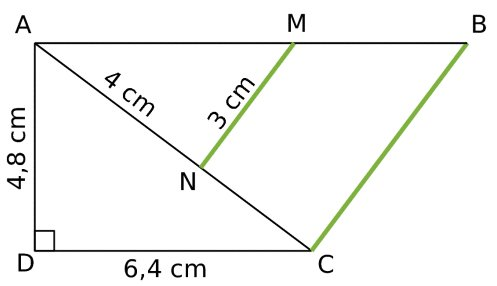
\includegraphics[width=6cm]{images/ex4.jpg}
\end{minipage}
\end{tabular}


\pagebreak


NOM PRENOM: \ldots \ldots \ldots \ldots \ldots

\begin{center}
{\fbox{$4^{e}3$ \qquad \qquad \textbf{\Large{Devoir surveill� 6 (sujet 2)}}
\qquad \qquad 15/04/2014}}
\end{center}


\textit{\ul{Remarque}: Les exercices 1 et 2 sont � faire sur la photocopie, les
autres sur votre copie.}

\enskip

\ul{\textbf{Exercice 1}}: (\textit{2 points})
\thinspace
Compl�ter le tableau suivant en arrondissant les valeurs au dixi�me.

\begin{center}
\begin{tabular}{|l|c|c|c|c|}
\hline
Angle & 65� & \ldots \ldots & 28� & \ldots \ldots \\
\hline

Cosinus & \ldots \ldots & 0,92 & \ldots \ldots & 0,5 \\
\hline
\end{tabular}
\end{center}

\bigskip

\ul{\textbf{Exercice 2}}: (\textit{2 points})
\thinspace 
Pour chaque question, coche la (ou les ) bonne(s) r�ponse(s).


\begin{center}
\begin{tabular}{|l|c|c|c|}
\hline


Dans un triangle RST rectangle en R, le c�t� adjacent � l'angle $\widehat{STR}$
est 

& [TS] & [SR] & [RT] \\

\quad & \fbox{\thinspace} & \fbox{\thinspace} & \fbox{\thinspace} \\

\hline

\quad & \quad & \quad & \quad \\
Dans un triangle ABC rectangle en B, $cos(\widehat{BAC})$ est �gal � 

& $\dfrac{BC}{AC}$ & $\dfrac{AB}{BC}$ & $\dfrac{AB}{AC}$ \\

\quad & \fbox{\thinspace} & \fbox{\thinspace} & \fbox{\thinspace} \\

\hline
\quad & \quad & \quad & \quad \\
Dans ce triangle rectangle, on peut calculer la valeur excate de 

& DE & $\widehat{DEF}$ & EF  \\

\quad & \fbox{\thinspace} & \fbox{\thinspace} & \fbox{\thinspace} \\

\hline
\end{tabular}
\end{center}


\bigskip


\ul{\textbf{Exercice 3}}: (\textit{2 points})



\begin{tabular}{cc}
\begin{minipage}{13cm}
Calculer la longueur NP. On donnera une valeur arrondie au millim�tre.
\end{minipage}
&
\begin{minipage}{5cm}
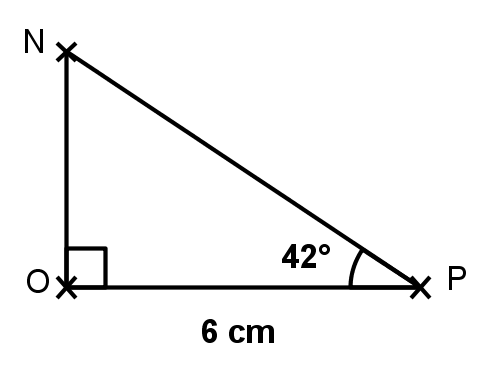
\includegraphics[width=4cm]{images/ex3-sujet2.png}
\end{minipage}
\end{tabular}


 
\medskip


\ul{\textbf{Exercice 4}}: (\textit{4 points})


\begin{tabular}{cc}
\begin{minipage}{14cm}
\begin{enumerate}
  \item Calculer la longueur ST. On donnera une valeur arrondie au centim�tre.
  \item Calculer la longueur RS. On donnera une valeur arrondie au centim�tre.
\end{enumerate}
\end{minipage}
&
\begin{minipage}{5cm}
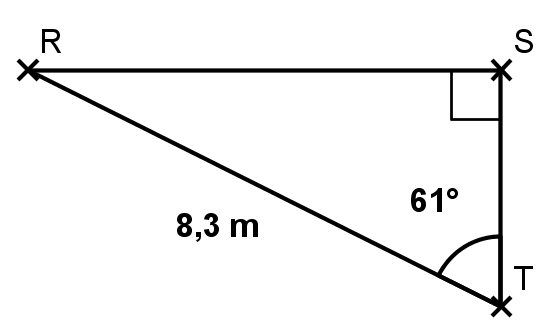
\includegraphics[width=4cm]{images/ex4-sujet2.png}
\end{minipage}
\end{tabular}


\medskip


\ul{\textbf{Exercice 5}}: (\textit{3 points})

\enskip 

KLM est un triangle rectangle en K v�rifiant KL=6km et LM=11km.
\begin{enumerate}
  \item Calculer la mesure de l'angle $\widehat{KLM}$. On donnera une valeur
  arrondie au degr�.
  \item En d�duire une mesure de l' angle $\widehat{KML}$. 
\end{enumerate}


\medskip



\ul{\textbf{Exercice 6}}: (\textit{7 points})

\enskip

\begin{tabular}{cc}
\begin{minipage}{12cm}

 Sur la figure ci-contre, les droites (MN) et (BC) sont parall�les et AB=10cm.
 
 \begin{enumerate}
   \item Montrer que AC=8cm. Justifier votre r�ponse.
   \item Calculer BC. Justifier votre r�ponse.
   
   \textbf{Pour la suite des questions, on admettra que BC=6cm.}
   
   
   \item Montrer que le triangle ABC est rectangle.
   \item Calculer la mesure de l'angle $\widehat{ABC}$. Arrondir au degr�.
   \item En d�duire une mesure de l'angle $\widehat{AMN}$.
 \end{enumerate}
\end{minipage}
&
\begin{minipage}{6cm}
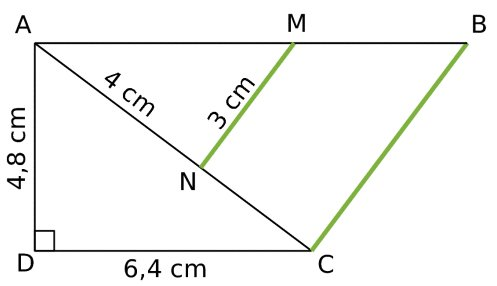
\includegraphics[width=6cm]{images/ex4.jpg}
\end{minipage}
\end{tabular}
\end{document}
